\begin{figure}[h!]
\centering
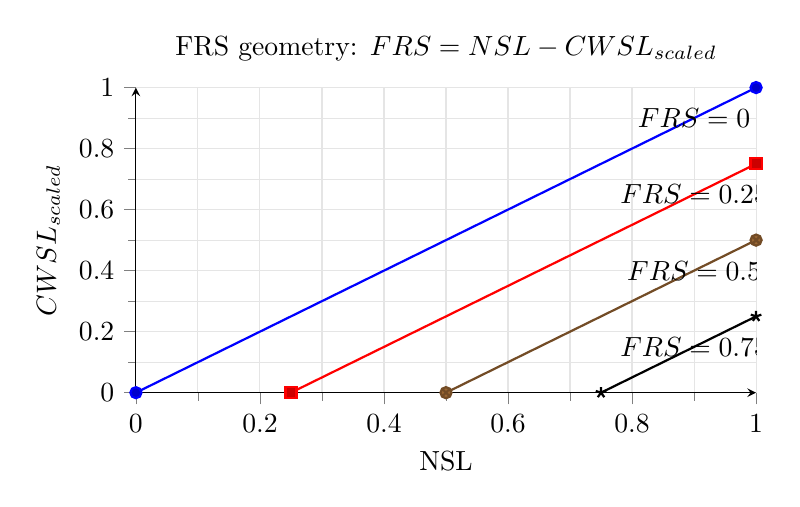
\begin{tikzpicture}

\begin{axis}[
    width=0.78\linewidth,
    height=0.45\linewidth,
    xmin=0, xmax=1,
    ymin=0, ymax=1,
    xlabel={NSL},
    ylabel={$CWSL_{\text{scaled}}$},
    axis lines=left,
    tick align=outside,
    grid=both,
    minor tick num=1,
    title={FRS geometry: $FRS = NSL - CWSL_{\text{scaled}}$},
    grid style={gray!20},
]

% Iso-FRS lines: CWSL_scaled = NSL - constant
\addplot+[domain=0:1, samples=2, thick] ({x},{x});
\addplot+[domain=0.25:1, samples=2, thick] ({x},{x - 0.25});
\addplot+[domain=0.5:1, samples=2, thick] ({x},{x - 0.5});
\addplot+[domain=0.75:1, samples=2, thick] ({x},{x - 0.75});

\node at (axis cs:0.9,0.9) {$FRS=0$};
\node at (axis cs:0.9,0.65) {$FRS=0.25$};
\node at (axis cs:0.9,0.4) {$FRS=0.5$};
\node at (axis cs:0.9,0.15) {$FRS=0.75$};

\end{axis}

\end{tikzpicture}

\caption{
FRS geometry as a function of NSL and $CWSL_{\text{scaled}}$. Diagonal level sets
represent constant values of $FRS = NSL - CWSL_{\text{scaled}}$, illustrating the
tradeoff between reliability and normalized cost.
}
\label{fig:frs_geometry}
\end{figure}